\begin{SCn}

\scnsectionheader{Предметная область и онтология логических формул, высказываний и логических онтологий}

\scnstartsubstruct

\scnheader{Предметная область логических формул, высказываний и логических онтологий}
\scniselement{предметная область}
\scnsdmainclasssingle{формальная теория}
\scnsdclass{высказывание;атомарное высказывание;неатомарное высказывание;фактографическое высказывание;логическая формула;атомарная логическая формула;неатомарная логическая формула;утверждение;определение;общезначимая логическая формула;противоречивая логическая формула;нейтральная логическая формула;выполнимая логическая формула;невыполнимая логическая формула;тавтология;логическая операция;квантор;формула существования;число значений переменной;кратность существования;единственное существование;логическая формула и единственность;открытая логическая формула;замкнутая логическая формула}
\scnsdrelation{предметная область’;аксиома’;теорема’;подформула*;импликация*;если’;то’;эквиваленция*;конъюнкция*;дизъюнкция*;строгая дизъюнкция*;отрицание*;всеобщность*;неатомарное существование*;связываемые переменные’}

\scnheader{формальная теория}
\scnexplanation{\textbf{\textit{формальная теория}} — это множество высказываний, которые считаются истинными в рамках данной \textbf{\textit{формальной теории}}. Высказывания могут быть как фактографическими, так и нет. Некоторые высказывания считаются аксиомами (не доказываются в рамках данной формальной теории), а другие доказываются на основе других высказываний в рамках этой же \textbf{\textit{формальной теории}}.

Каждая формальная теория интерпретируется (т.е. ее высказывания являются истинными) на какой-либо \textit{предметной области}, которая является максимальным из \textit{фактографических высказываний} (их объединением*), входящих в состав этой \textbf{\textit{формальной теории}}. Каждой \textbf{\textit{формальной теории}} соответствует одна \textit{предметная область}, которая входит в нее под атрибутом \textit{предметная область'}.

Каждая \textbf{\textit{формальная теория}} может рассматриваться как \textit{конъюнктивное высказывание}, априори истинное (с чьей-то точки зрения) при интерпретации на соответствующей \textit{предметной области}.}

\scnheader{предметная область’}
\scniselement{ролевое отношение}
\scnexplanation{\textbf{\textit{предметная область’}} – это \textit{ролевое отношение}, связывающее \textit{формальную теорию} с \textit{предметной областью}, на которой данная \textit{формальная теория} интерпретируется (в рамках которой истинны \textit{высказывания}, входящие в состав этой \textit{формальной теории}). Другими словами, эта \textit{предметная область} является максимальным фактографическим высказыванием этой \textit{формальной теории}.}

\scnheader{аксиома’}
\scniselement{ролевое отношение}
\scnexplanation{\textbf{\textit{аксиома’}} – это \textit{ролевое отношение}, связывающее \textit{формальную теорию} с \textit{высказыванием}, истинность которого не доказывается в её рамках.}

\scnheader{теорема’}
\scniselement{ролевое отношение}
\scnexplanation{\textbf{\textit{теорема’}} – это \textit{ролевое отношение}, связывающее \textit{формальную теорию} с \textit{высказыванием}, истинность которого доказывается в её рамках.}

\scnheader{высказывание}
\scnsubset{структура}
\scnreltoset{разбиение}{атомарное высказывание;неатомарное высказывание}
\scnreltoset{разбиение}{фактографическое высказывание;логическая формула}
\scnexplanation{Под \textbf{\textit{высказыванием}} понимается некоторая \textit{структура}, которая может трактоваться как истинная или ложная в рамках какой-либо \textit{предметной области}. Истинность \textbf{\textit{высказывания}} задается путем указания принадлежности знака этого высказывания \textit{формальной теории}, соответствующей данной \textit{предметной области}. Ложность высказывания задается путем указания принадлежности знака \textit{отрицания*} этого высказывания данной \textit{формальной теории}. Явно указанная непринадлежность \textbf{\textit{высказывания}} \textit{формальной теории} может говорить как о его ложности в рамках данной теории (если это указано рассмотренным выше образом), так и о том, что дано \textbf{\textit{высказывание}} вообще не рассматривается в данной \textit{формальной теории} (например, использует понятия, не принадлежащие данной \textit{предметной области}). 

Одно и то же \textbf{\textit{высказывание}} может быть истинно в рамках одной \textit{формальной теории} и ложно в рамках другой.

Каждое высказывание может либо содержать \textit{sc-элементы}, которые не являются знаками других \textbf{\textit{высказываний}} (быть атомарным), либо содержать только знаки других \textbf{\textit{высказываний}} (быть неатомарным).}

\scnheader{атомарное высказывание}
\scnexplanation{\textbf{\textit{атомарное высказывание}} – это \textit{высказывание}, которое содержит хотя бы один \textit{sc-элемент}, не являющийся знаком другого \textit{высказывания}.}

\scnheader{неатомарное высказывание}
\scnexplanation{\textbf{\textit{неатомарное высказывание}} – это \textit{высказывание}, в состав которого входят только знаки других \textit{высказываний}.

Следует отметить, что мы не можем говорить об истинности либо ложности \textbf{\textit{неатомарного высказывания}} в рамках какой-либо \textit{формальной теории}, в случае, когда невозможно установить истинность либо ложность любого из его элементов в рамках этой же \textit{формальной теории}.}

\scnheader{фактографическое высказывание}
\scnexplanation{Под \textit{фактографическим высказыванием} понимается:
\begin{scnitemize}
    \item \textit{атомарное высказывание}, в состав которого не входит ни одна \textit{sc-переменная};
    \item \textit{неатомарное высказывание}, все элементы которого также являются \textbf{\textit{фактографическими высказываниями}}.
\end{scnitemize}
}

\scnheader{логическая формула}
\scnexplanation{Под \textit{логической формулой} понимается:
\begin{scnitemize}
    \item \textit{атомарное высказывание}, в состав которого входит хотя бы одна \textit{sc-переменная};
    \item \textit{неатомарное высказывание}, хотя бы один элемент которого является \textbf{\textit{логической формулой}}.
\end{scnitemize}}
\scnreltoset{разбиение}{атомарная логическая формула;неатомарная логическая формула}
\scnreltoset{разбиение}{открытая логическая формула;замкнутая логическая формула}

\scnheader{атомарная логическая формула}
\scnidtf{обобщенная структура}
\scnidtf{атомарная формула существования}
\scnexplanation{Под \textbf{\textit{атомарной логической формулой}} понимается \textit{атомарное высказывание}, которое является \textit{логической формулой}.

По умолчанию \textbf{\textit{атомарная логическая формула}} трактуется как \textit{высказывание} о существовании, то есть наличия в памяти значений, соответствующих всем \textit{sc-переменным}, входящим в состав данной формулы и не попадающих под действие какого-либо другого \textit{квантора} (указанного явно или по умолчанию). Таким образом, на все \textit{sc-переменные}, входящие в состав \textbf{\textit{атомарной логической формулы}}, и не попадающие под действие какого-либо другого \textit{квантора}, неявно накладывается квантор \textit{существования*}.}

\scnheader{неатомарная логическая формула}
\scnreltoset{разбиение}{общезначимая логическая формула;противоречивая логическая формула;нейтральная логическая формула}
\scnreltoset{разбиение}{выполнимая логическая формула;невыполнимая логическая формула}
\scnsuperset{тавтология}
\scnexplanation{Под \textbf{\textit{неатомарной логической формулой}} понимается \textit{неатомарное высказывание}, которое является \textit{логической формулой}.

Для того, чтобы рассмотреть типологию \textbf{\textit{неатомарных логических формул}}, будем говорить, что исследуется истинность самой \textbf{\textit{неатомарной логической формулы}} и всех ее \textit{подформул*} в рамках одной и той же \textit{формальной теории}, при этом не важно, какой именно. Также считается, что в рассматриваемой \textit{формальной теории} каждая \textit{подформула*} рассматриваемой \textbf{\textit{неатомарной логической формулы}} является в рамках этой \textit{формальной теории} может однозначно трактоваться как либо истинная, либо ложная. В противном случае мы не можем говорить об истинности либо ложности исходной \textbf{\textit{неатомарной логической формулы}} в рамках этой \textit{формальной теории}.}

\scnheader{подформула*}
\scnidtf{частная формула*}
\scniselement{бинарное отношение}
\scniselement{ориентированное отношение}
\scniselement{транзитивное отношение}
\scntext{определение}{Будем называть \textbf{\textit{подформулой*}} \textit{неатомарной логической формулы} любую \textit{логическую формулу}, являющуюся элементом исходной формулы, а также любую \textbf{\textit{подформулу*}} \textit{неатомарной логической формулы}, являющейся элементом исходной \textit{неатомарной логической формулы}.

Будем также считать исходную \textit{логическую формулу} \textbf{\textit{подформулой*}} самой себя.}

\scnheader{утверждение}
\scnidtf{текст логической формулы}
\scntext{определение}{\textbf{\textit{утверждение}} – это \textit{семантическая окрестность} некоторой \textit{логической формулы}, в которую входит полный текст этой \textit{логической формулы}, а также факт принадлежности этой \textit{логической формулы} некоторой \textit{формальной теории}. Знак указанной \textit{логической формулы} является \textit{главным ключевым sc-элементом'} в рамках этого \textbf{\textit{утверждения}}. Знаки понятий соответствующей \textit{предметной области}, которые входят в состав какой-либо \textit{подформулы*} указанной \textit{логической формулы}, будут \textit{ключевыми sc-элементами'} в рамках этого \textbf{\textit{утверждения}}.

Полный текст некоторой \textit{логической формулы} включает в себя:
\begin{scnitemize}
    \item знак самой этой \textit{логической формулы};
    \item знаки всех ее \textit{подформул*};
    \item элементы всех \textit{логических формул}, знаки которых попали в данную структуру;
    \item все пары принадлежности, связывающие \textit{логические формулы}, знаки которых попали в данную структуру, с их компонентами.
\end{scnitemize}
Таким образом, факт принадлежности (истинности) логической формулы нескольким \textit{формальным теориям} будет порождать новое утверждение для каждой такой \textit{формальной теории}. Текст \textbf{\textit{утверждения}} входит в состав \textit{логической онтологии}, соответствующей \textit{предметной области}, на которой интерпретируется \textit{главный ключевой sc-элемент'} данного утверждения.}
\scntext{правило идентификации экземпляров}{\textbf{\textit{утверждения}} в рамках \textit{Русского языка} именуются по следующим правилам:
\begin{scnitemize}
    \item в начале идентификатора пишется сокращение \textbf{Утв.};
    \item далее в круглых скобках через точку с запятой перечисляются основные идентификаторы \textit{ключевых sc-элементов'} данного \textbf{\textit{утверждения}}. Порядок определяется в каждом конкретном случае в зависимости от того, свойства каких из этих \textit{понятий} описывает данное \textbf{\textit{утверждение}} в большей или меньшей степени.
\end{scnitemize}
Например:\\
\textit{Утв. (треугольник, сторона*)}

Могут быть исключения для \textbf{\textit{утверждений}}, названия которых закрепились исторически, например, \textit{Теорема Пифагора}, \textit{Аксиома о прямой и точке}.}

\scnheader{определение}
\scnidtf{текст определения}
\scnsubset{утверждение}
\scntext{определение}{\textbf{\textit{определение}} – это \textit{утверждение}, \textit{главным ключевым sc-элементом’} которого является связка \textit{эквиваленции*}, однозначно определяющая некоторое понятие соответствующее понятие на основе других. Таким образом, каждое определение имеет ровно один \textit{ключевой sc-элемент’} (не считая \textit{главного ключевого sc-элемента’}).

Следует отметить, что для одного и того же понятия в рамках одной \textit{формальной теории} может существовать несколько \textit{утверждений об эквиваленции*}, однозначно задающих некоторое понятие на основе других, однако только одно такое \textit{утверждение} в рамках этой \textit{формальной теории} может быть отмечено как \textbf{\textit{определение}}.}
\scntext{правило идентификации экземпляров}{\textbf{\textit{определения}} в рамках \textit{Русского языка} именуются по следующим правилам:
\begin{scnitemize}
    \item в начале идентификатора пишется сокращение \textbf{Опр.};
    \item далее в круглых скобках через точку с запятой записывается основной идентификатор  \textit{ключевого sc-элемента'} данного \textbf{\textit{определения}}.
\end{scnitemize}
Например:\\
\textit{Опр. (связный граф)}
}

\scnheader{общезначимая логическая формула}
\scnsubset{выполнимая логическая формула}
\scnsubset{тавтология}
\scntext{определение}{\textbf{\textit{общезначимая логическая формула}} – это \textit{неатомарная логическая формула}, для которой не существует \textit{формальной теории}, в рамках которой она была бы ложной с учетом истинности и ложности всех ее \textit{подформул*} в рамках этой же \textit{формальной теории}.}

\scnheader{противоречивая логическая формула}
\scnsubset{невыполнимая логическая формула}
\scnsubset{тавтология}
\scntext{определение}{\textbf{\textit{противоречивая логическая формула}} – это \textit{неатомарная логическая формула}, для которой не существует \textit{формальной теории}, в рамках которой она была бы истинной с учетом истинности и ложности всех ее \textit{подформул*} в рамках этой же \textit{формальной теории}.}

\scnheader{нейтральная логическая формула}
\scnsubset{выполнимая логическая формула}
\scntext{определение}{\textbf{\textit{нейтральная логическая формула}} – это \textit{неатомарная логическая формула}, для которой существует хотя бы одна \textit{формальная теория}, в рамках которой эта формула ложна и хотя бы одна \textit{формальная теория}, в рамках которой эта формула истинна.}

\scnheader{выполнимая логическая формула}
\scntext{определение}{\textbf{\textit{выполнимая логическая формула}} – это \textit{неатомарная логическая формула}, для которой существует хотя бы одна \textit{формальная теория}, в рамках которой эта формула истинна.}

\scnheader{невыполнимая логическая формула}
\scntext{определение}{\textbf{\textit{невыполнимая логическая формула}} – это \textit{неатомарная логическая формула}, для которой существует хотя бы одна \textit{формальная теория}, в рамках которой эта формула ложна.}

\scnheader{тавтология}
\scnidtf{тождественно истинная формула}
\scntext{определение}{\textbf{\textit{тавтология}} – это \textit{неатомарная логическая формула}, которая является либо \textit{общезначимой логической формулой}, либо \textit{противоречивой логической формулой}. Другими словами, это такая \textit{неатомарная логическая формула}, которая является либо только истинной, либо только ложной в рамках всех \textit{формальных теорий}, в которых можно установить ее истинность или ложность.}

\scnheader{логическая операция}
\scnidtf{класс неатомарных высказываний}
\scnidtf{логическая связка}
\scnidtf{логический оператор}
\scnidtf{пропозициональная связка}
\scnrelto{семейство подмножеств}{неатомарное высказывание}
\scnexplanation{\textbf{\textit{логическая операция}} – это класс \textit{неатомарных высказываний}. Другими словами это \textit{отношение}, областью определения которого является множество \textit{высказываний}, при этом некоторые из таких \textit{отношений} могут быть \textit{классами связок разной мощности}.}

\scnheader{импликация*}
\scnidtf{логическое следование*}
\scniselement{логическая операция}
\scniselement{бинарное отношение}
\scniselement{ориентированное отношение}
\scntext{определение}{\textbf{\textit{импликация*}} - это множество импликативных \textit{неатомарных высказываний}, каждое из которых состоит из посылки (первый компонент \textit{высказывания}) и следствия (второй компонент \textit{высказывания}). Каждое импликативное \textit{высказывание} ложно в рамках некоторой \textit{формальной теории} в том случае, когда его посылка истинна, а заключение ложно в рамках этой же \textit{формальной теории}. В других случаях такое \textit{высказывание} истинно.

По умолчанию на все переменные, входящие в обе части высказывания об \textbf{\textit{имликации*}} (или хотя бы одну из \textit{подформул*} каждой части) неявно накладывается квантор \textit{всеобщности*}, при условии, что эти переменные не связаны другим \textit{квантором}, указанным явно.}
\scnrelfrom{описание типичного экземпляра}{
\scnfilelong{
\begin{figure}[H]
\centering
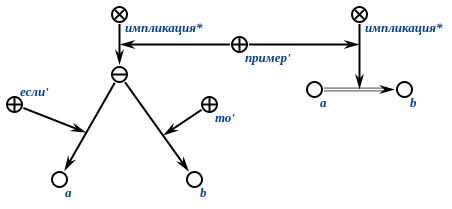
\includegraphics[width=1\linewidth]{figures/sd_logical_formulas/implication.png}
\end{figure}
}}

\scnheader{если’}
\scnsubset{1'}
\scniselement{ролевое отношение}
\scntext{определение}{\textbf{\textit{если’}} - это \textit{ролевое отношение}, используемое в связках \textit{импликации*}, для указания посылки.}
\scnrelfrom{описание типичного экземпляра}{
\scnfilelong{
\begin{figure}[H]
\centering
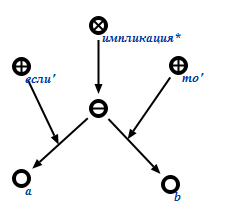
\includegraphics[width=0.5\linewidth]{figures/sd_logical_formulas/if.png}
\end{figure}
}}

\scnheader{то’}
\scnsubset{2'}
\scniselement{ролевое отношение}
\scntext{определение}{\textbf{\textit{то’}} - это \textit{ролевое отношение}, используемое в связках \textit{импликации*}, для указания следствия.}
\scnrelfrom{описание типичного экземпляра}{
\scnfilelong{
\begin{figure}[H]
\centering
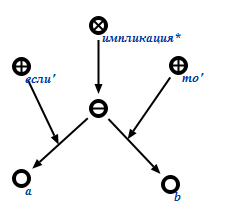
\includegraphics[width=0.5\linewidth]{figures/sd_logical_formulas/then.png}
\end{figure}
}}

\scnheader{эквиваленция*}
\scnidtf{эквиваленция*}
\scniselement{логическая операция}
\scniselement{бинарное отношение}
\scniselement{неориентированное отношение}
\scntext{определение}{\textbf{\textit{эквиваленция*}} - это множество \textit{неатомарных высказываний} об эквивалентности, каждое из которых истинно в рамках некоторой \textit{формальной теории} только в тех случаях, когда оба его компонента одновременно либо истинны в рамках этой же \textit{формальной теории}, либо ложны.

По умолчанию на все переменные, входящие в обе части высказывания об \textbf{\textit{эквиваленции*}} (или хотя бы одну из \textit{подформул*} каждой части) неявно накладывается квантор \textit{всеобщности*}, при условии, что эти переменные не связаны другим \textit{квантором}, указанным явно.}
\scnrelfrom{описание типичного экземпляра}{
\scnfilelong{
\begin{figure}[H]
\centering
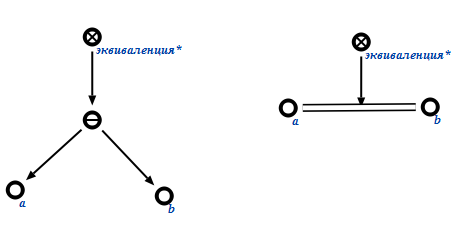
\includegraphics[width=1\linewidth]{figures/sd_logical_formulas/equivalent.png}
\end{figure}
}}

\scnheader{конъюнкция*}
\scnidtf{логическое и*}
\scnidtf{логическое умножение*}
\scniselement{логическая операция}
\scniselement{неориентированное отношение}
\scnsubset{класс связок разной мощности}
\scntext{определение}{\textbf{\textit{конъюнкция*}} - это множество конъюнктивных \textit{высказываний}, каждое из которых истинно в рамках некоторой \textit{формальной теории} только в том случае, когда все его компоненты истинны в рамках этой же \textit{формальной теории}.}
\scnrelfrom{описание типичного экземпляра}{
\scnfilelong{
\begin{figure}[H]
\centering
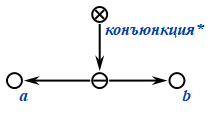
\includegraphics[width=0.5\linewidth]{figures/sd_logical_formulas/conjunction.png}
\end{figure}
}}

\scnheader{дизъюнкция*}
\scnidtf{логическое или*}
\scnidtf{логическое сложение*}
\scnidtf{включающее или*}
\scniselement{логическая операция}
\scniselement{неориентированное отношение}
\scnsubset{класс связок разной мощности}
\scntext{определение}{\textbf{\textit{дизъюнкция*}} - это множество дизъюнктивных \textit{высказываний}, каждое из которых истинно в рамках некоторой \textit{формальной теории} только в том случае, когда хотя бы один его компонент является истинным в рамках этой же \textit{формальной теории}.}
\scnrelfrom{описание типичного экземпляра}{
\scnfilelong{
\begin{figure}[H]
\centering
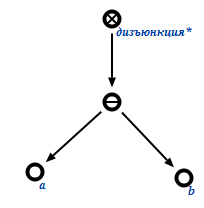
\includegraphics[width=0.5\linewidth]{figures/sd_logical_formulas/disjunction.png}
\end{figure}
}}

\scnheader{строгая дизъюнкция*}
\scnidtf{сложение по модулю 2*}
\scnidtf{исключающее или*}
\scnidtf{альтернатива*}
\scniselement{логическая операция}
\scniselement{неориентированное отношение}
\scnsubset{класс связок разной мощности}
\scntext{определение}{\textbf{\textit{строгая дизъюнкция*}} - это множество строго дизъюнктивных \textit{высказываний}, каждое из которых истинно в рамках некоторой \textit{формальной теории} только в том случае, когда ровно один его компонент является истинным в рамках этой же \textit{формальной теории}.}
\scnrelfrom{описание типичного экземпляра}{
\scnfilelong{
\begin{figure}[H]
\centering
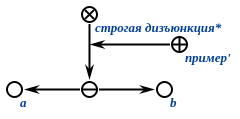
\includegraphics[width=0.5\linewidth]{figures/sd_logical_formulas/strictDisjunction.png}
\end{figure}
}}

\scnheader{отрицание*}
\scniselement{логическая операция}
\scnsubset{синглетон}
\scntext{определение}{\textbf{\textit{отрицание*}} - это множество \textit{высказываний} об отрицании, каждое из которых истинно в рамках некоторой \textit{формальной теории} только в том случае, когда его единственный элемент является ложным в рамках этой же \textit{формальной теории}.}

\scnheader{квантор}
\scnsubset{логическая операция}
\scntext{определение}{\textbf{\textit{квантор}} – это \textit{логическая операция}, каждая связка которой задает истинность множества \textit{логических формул}, входящих в ее состав, при выполнении дополнительных условий, связанных с некоторыми из переменных, входящих в состав этих \textit{логических формул}. Будем говорить, что указанные переменные связаны \textbf{\textit{квантором}} или попадают под область действия данного \textbf{\textit{квантора}} (имея в виду конкретную связку конкретного \textbf{\textit{квантора}}). Таким образом, в состав каждой связки каждого \textbf{\textit{квантора}} входит \textit{атомарная формула}, являющаяся \textit{тривиальной структурой}, в которой перечислены переменные, связанные данным \textbf{\textit{квантором}}.}

\scnheader{всеобщность*}
\scnidtf{квантор всеобщности*}
\scnidtf{квантор общности*}
\scniselement{квантор}
\scniselement{ориентированное отношение}
\scnsubset{класс связок разной мощности}
\scntext{определение}{\textbf{\textit{всеобщность}} – это \textit{квантор}, для каждой связки которого, истинной в рамках некоторой \textit{формальной теории}, выполняется следующее утверждение: все формулы, входящие в состав этой связки истинны в рамках этой же \textit{формальной теории} при всех (любых) возможных значениях всех элементов множества \textit{связываемых переменных'} входящего в эту связку.

Каждая связка \textit{квантора} \textbf{\textit{всеобщность*}} может быть представлена как \textit{конъюнкция*} (потенциально бесконечная) исходных \textit{логических формул}, входящих в состав этой связки, в каждой из которых все \textit{связанные переменные'} заменены на их возможные значения.}
\scnrelfrom{описание типичного экземпляра}{
\scnfilelong{
\begin{figure}[H]
\centering
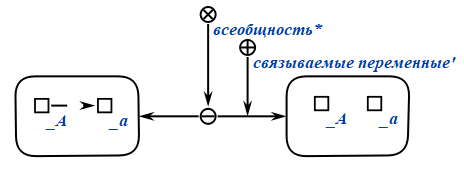
\includegraphics[width=0.8\linewidth]{figures/sd_logical_formulas/universality.png}
\end{figure}
}}

\scnheader{формула существования}
\scnidtf{существование*}
\scnreltoset{разбиение}{атомарная логическая формула;неатомарное существование*}

\scnheader{неатомарное существование*}
\scnidtf{квантор неатомарного существования*}
\scniselement{квантор}
\scniselement{ориентированное отношение}
\scnsubset{класс связок разной мощности}
\scntext{определение}{\textbf{\textit{неатомарное существование*}} – это \textit{квантор}, для каждой связки которого, истинной в рамках некоторой \textit{формальной теории}, выполняется следующее утверждение: существуют значения всех элементов множества \textit{связываемых переменных'} входящего в эту связку, такие, что все формулы, входящие в состав этой связки истинны в рамках этой же \textit{формальной теории}.

Каждая связка \textit{квантора} \textbf{\textit{неатомарное существование*}} может быть представлена как \textit{дизъюнкция*} (потенциально бесконечная) исходных \textit{логических формул}, входящих в состав этой связки, в каждой из которых все \textit{связанные переменные'} заменены на их возможные значения.}
\scnrelfrom{описание типичного экземпляра}{
\scnfilelong{
\begin{figure}[H]
\centering
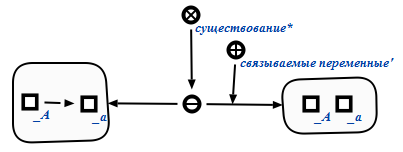
\includegraphics[width=0.8\linewidth]{figures/sd_logical_formulas/non_atomicExistence.png}
\end{figure}
}}

\scnheader{число значений переменной}
\scniselement{параметр}
\scnexplanation{Каждый элемент \textit{параметра} \textbf{\textit{число значений переменной}} представляет собой класс ориентированных пар, первым компонентом которых является знак \textit{логической формулы}, вторым – \textit{sc-переменная}, имеющая в рамках данной \textit{логической формулы} ограниченное известное число значений, при которых данная формула является истинной в рамках соответствующей \textit{формальной теории}.\\
Отметим, что в случае \textit{атомарной логической формулы} каждая такая связка связывает знак формулы и знак принадлежащей ей \textit{sc-переменной}, т.е. является, по сути, частным случаем пары принадлежности. В случае \textit{неатомарной логической формулы} указанная \textit{sc-переменная} может принадлежать любой из \textit{подформул*} исходной формулы.

Таким образом, \textit{измерением*} каждого значения параметра \textbf{\textit{число значений переменной}} является некоторое \textit{число}, задающее количество значений \textit{sc-переменных} в рамках \textit{логической формулы}.}

\scnheader{кратность существования}
\scniselement{параметр}
\scnrelfrom{область определения параметра}{формула существования}
\scnhaselement{единственное существование}
\scnexplanation{Каждый элемент \textit{параметра} \textbf{\textit{кратность существования}} представляет собой класс логических \textit{формул существования}, для которых  при интерпретации на соответствующей \textit{предметной области} существует ограниченное общее для всех таких формул число комбинаций значений переменных, при которых указанные формулы являются истинными в рамках соответствующей \textit{формальной теории}.

Таким образом, \textit{измерением*} каждого значения \textbf{\textit{кратности существования}} является некоторое \textit{число}, задающее количество таких комбинаций.}

\scnheader{единственное существование}
\scnidtf{однократное существование}
\scnidtf{формула существования и единственности}

\scnheader{логическая формула и единственность}
\scnsubset{логическая формула}
\scnsubset{единственное существование}
\scnexplanation{Каждый элемент множества \textbf{\textit{логическая формула и единственность}} представляет собой \textit{логическую формулу} (\textit{атомарную} или \textit{неатомарную}), для которой дополнительно уточняется, что при ее интерпретации на некоторой предметной области существует только один набор значений переменных, входящих в эту формулу (или ее \textit{подформулы*}), при котором указанная логическая формула истинна в рамках \textit{формальной теории}, в которую входит данная \textit{предметная область}.}

\scnheader{связываемые переменные’}
\scniselement{ролевое отношение}
\scntext{определение}{\textbf{\textit{связываемые переменные’}} – это \textit{ролевое отношение}, которое связывает связку конкретного \textit{квантора} с множеством переменных, которые связаны этим квантором.}
\scnrelfrom{описание типичного экземпляра}{
\scnfilelong{
\begin{figure}[H]
\centering
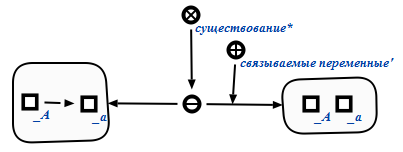
\includegraphics[width=0.8\linewidth]{figures/sd_logical_formulas/bindVariables.png}
\end{figure}
}}

\scnheader{открытая логическая формула}
\scntext{определение}{\textbf{\textit{открытая логическая формула}} – это \textit{логическая формула}, в рамках которой (и всех ее \textit{подформул*}) существует хотя бы одна переменная, не связанная никаким \textit{квантором}.}

\scnheader{замкнутая логическая формула}
\scntext{определение}{\textbf{\textit{замкнутая логическая формула}} – это \textit{логическая формула}, в рамках которой (и всех ее \textit{подформул*}) не существует переменных, не связанных каким-либо \textit{квантором}.}

\scnendstruct

\end{SCn}